\documentclass[a4paper]{article}

\usepackage{microtype}
\usepackage[T1]{fontenc}
\usepackage[hmarginratio=1:1,top=32mm,margin=2cm]{geometry}

\usepackage{graphicx}
\usepackage{todonotes}
\usepackage{hyperref}

\usepackage{amsmath}
\usepackage{algorithm}
\usepackage[noend]{algpseudocode}

\makeatletter
\algrenewcommand\ALG@beginalgorithmic{\small}
\makeatother


\title{HumHub custom specifications}
\author{Francesco Bailo \href{mailto:francesco.bailo@sydney.edu.au}{francesco.bailo@sydney.edu.au}}
\date{\today\\v2}

\begin{document}

\maketitle

\section{Changes}
  \begin{description}
  \item [Added] Pseudocode for Algorithm~\ref{algo:filterStream} and Algorithm~\ref{algo:inferContentPolOp}
   \item [Added] more details in Section~\ref{sec:filtering}
  \end{description}

\section{Introduction}

I will use the ``Social Network Kit'' \href{https://www.humhub.org/}{HumHub} to run an online experiment. The experiment will provide behavioural data to measure the effect on exposure to political content representing specific political views.

\section{Definitions and abbreviations}

These definitions are based on (my understanding of) the \href{http://docs.humhub.org/index.html}{documentation} of HumHub and on the requirements for the project.

\begin{description}

\item[Social networking site] (SNS) is the online platform based on the HubHub framework where the experiment will take place. It will be hosted on servers administered by the \href{https://nectar.org.au/research-cloud/}{Nectar research cloud} (NRC) and on servers administered by the University of Sydney (USYD).

\item[Preliminary survey] Each user will complete a survey before signing up with the SNS. The survey will be used to quantify users' political views. The online survey will be administered externally with RedCap. 

\item[User] Each user will need to be characterised according to his/her \textit{political orientation} and \textit{topic interest}. \textit{Political orientation} will be captured by variables coded after the completion of a preliminary surveys. There will be a general political orientation variable and variables quantifying political opinion for each topic (see Table~\ref{tab:topics} for a list of topics). For each defined topic, a user will also have a variable defining his/her interest. These variables will be coded based on the observed behaviour of the user (see Table~\ref{tab:type_variables} for a list of user variable types).

  \item[Variable] A variable is stored in a database field: $variable==field$.
  
\item[Topic] A topic is a tag associated to a content entry. It is defined by the author of the content entry (either a user or an administrator). The complete list of topics is presented in Table~\ref{tab:topics}.

\item[Content entry] A content entry contains text, images or links to some resource (internal or external). It is published by a user or by an administrator. Each content entry will be quantified by at least one topic. Each content entry will be qualified 

\item[Stream] A stream is an ordered series of content entries.

\item[Dashboard] The dashboard is the timeline of a user. It must be always the first visible tab when a user log in.
  
\end{description}

\begin{table}[]
  \centering
\begin{tabular}{cc}
\textbf{Abbreviation} & \textbf{Description} \\ \hline
\verb|abo| & Abortion                   \\
\verb|imm| & Immigration                \\
\verb|gay| & LGBT rights                \\
\verb|eco| & Economic governance        \\
\verb|cli| & Climate change            
\end{tabular}
\caption{List of topics: abbreviations and description}
\label{tab:topics}
\end{table}

\begin{table}[]
    \centering
\begin{tabular}{cp{3.5cm}cp{3.5cm}}
\textbf{Abbreviation} & \textbf{Description} & \textbf{Data type} & \textbf{Scope} \\ \hline
\verb|pol_op| & Political opinion & double & It can be followed by a topic label. Alone, it refers to \textit{general} political opinion. \\
\verb|int_sur| & Political interest  as captured by survey responses & double & Always followed by a topic label  \\
\verb|int_obs| & Political interest as captured by SNS observation & double & Always followed by a topic label       
\end{tabular}
\caption{Types of variables: abbreviations and description}
\label{tab:type_variables}
\end{table}

\section{Processes}

The class \verb|user| will be modified based on what described in Figure~\ref{fig:class_diagram}. All the new variables with prefix \verb|pol_op| and suffix \verb|sur| are \verb|set()| after the completion of the survey. All the new variables with suffix \verb|obs| are updated following the activity of the user.

\begin{figure}
    \centering
    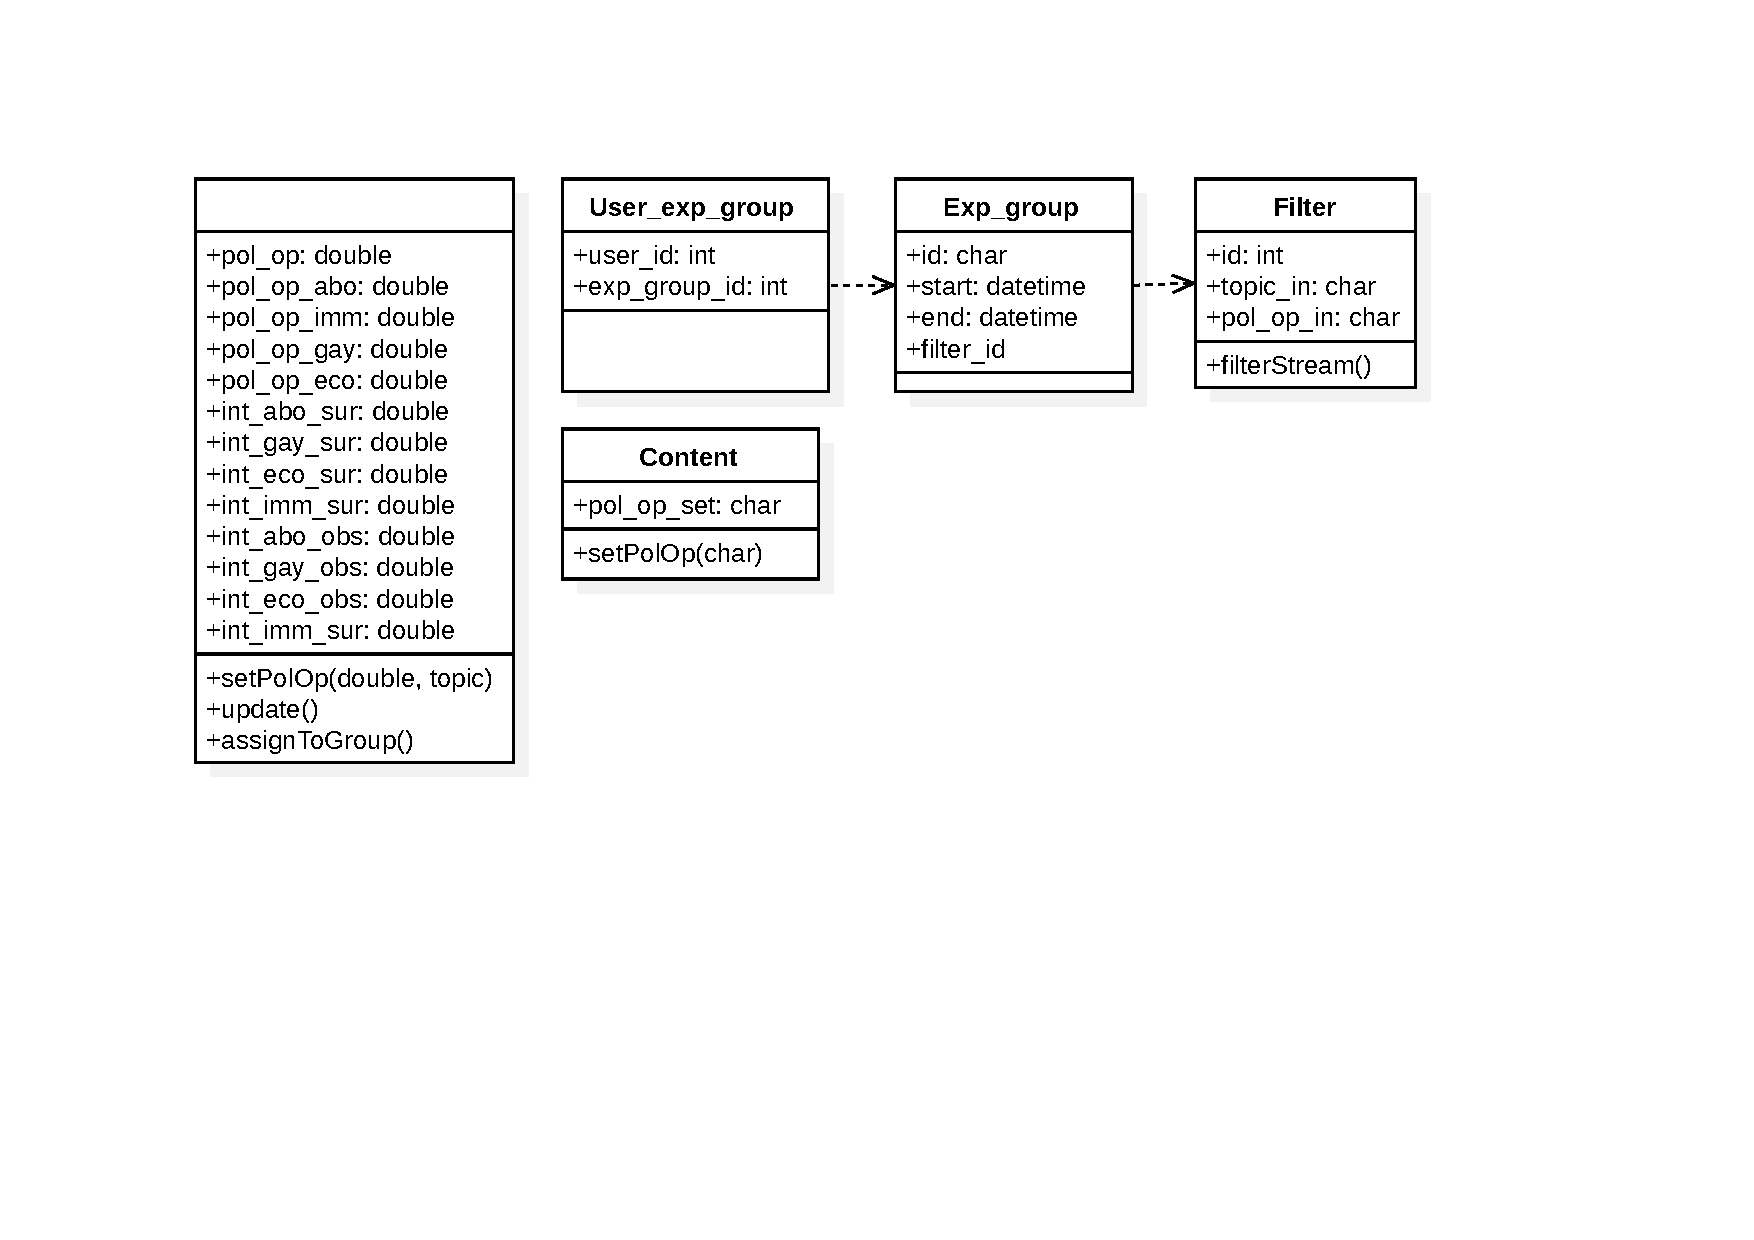
\includegraphics[width=\linewidth]{class_diagram}
    \caption{New or modified classes}
    \label{fig:class_diagram}
  \end{figure}

  \todo[inline, backgroundcolor=yellow]{Note: \texttt{set()} and \texttt{assignToGroup()} can be performed externally. That is, the developer doesn't need to write functions or create a web interface. I just need to know which SQL commands I can \textit{safely} execute on the SNS database.}

  \todo[inline, backgroundcolor=red!50!white]{To do: \texttt{update()} will need to be implemented by the developer.}

  \todo[inline, backgroundcolor=red!50!white]{To do: During an experiment \texttt{obs} variables are not updated.}

 \subsection{Content}

 Each content is described by an object of class \verb|topic| and by one new variable capturing the political opinion as defined \textit{directly} by the administrator when posting the content. \verb|pol_op_set| that takes two values (\verb|left| and \verb|right|). 

 \todo[inline, backgroundcolor=yellow]{Note: The manipulation of the \texttt{content} objects can be performed externally. Although it would be useful if the administrator could select \texttt{left} or \texttt{right} when creating a new content.}
 
  \subsection{Experiment set up}

When an experiment is set up, two objects of class \verb|exp_group| are (manually) created and stored in the corresponding table under the same \verb|id|, one for the \textit{treatment group} and one for the \textit{control group}. The table \verb|exp_group| primary key consists of two fields: \verb|id| and \verb|group_type|. The field \verb|group_type| can only take two values: \verb|treatment| and \verb|control|. 

When a user is (manually) assigned to an experiment, a corresponding object of class \verb|user_id| is stored into the table \verb|user_exp_group|.

 \todo[inline, backgroundcolor=yellow]{Note: The manipulation of objects of class \texttt{user\_exp\_group}, \texttt{exp\_group} and  \texttt{filter} can be performed externally.}

\subsection{Filtering}\label{sec:filtering}

Each user assigned to a group (\verb|exp_group|) of an ongoing experiment, will have his/her dashboard filtered by the function \verb|filterStream()| according to what set in the corresponding object of class \verb|filter|. An object of class \verb|filter| is characterised by a variable \verb|topic_in|, defining the single topic that must be given preference. \verb|topic_in| can assume as value any of the topic labels defined in Table~\ref{tab:topics} and the is nullable if no preference is to be given to a specific topic. \verb|pol_op_in| can assume two values: \verb|left| and \verb|right| and it is nullable if no preference is to be given on the political opinion of the content.

\subsubsection{filterStream()}

The function \verb|filterStream|is the core function for the administration of the experiment. It takes two objects: an object \verb|this_filter| of the class \verb|filter| and an array \verb|stream| of objects of class \verb|content|. The function determines what a user participating to an experiment see on his/her Dashboard.

The function \verb|filterStream| calls these other functions that, if not otherwise specified, consist of a simple SQL query:

\begin{itemize}
\item \verb|getTopicIn()| accesses the \verb|Filter| table.
\item \verb|getPolOpIn()| accesses the \verb|Filter| table.
\item \verb|getContentTopic()| accesses the \verb|Topic| table.
\item \verb|getContentPolOpSet()| accesses the \verb|Topic| table.
\item \verb|getAuthor()| accesses the \verb|Topic| table and return the author id.
\item  \verb|getAuthorPolOp()| accesses the \verb|User| table.
\item \verb|getAuthorPolOpTopic()| accesses the \verb|User| table.
\item \verb|getContentLikers()| access the \verb|Like| table.
  \end{itemize}

\begin{algorithm}
\caption{Stream filtering}\label{algo:filterStream}
\begin{algorithmic}[1]
  \Procedure{filterStream}{\texttt{stream}, \texttt{this\_filter}}
  \State $\texttt{filter\_topic\_in} \gets \text{getTopicIn}(\texttt{this\_filter})$
  \State $\texttt{filter\_pol\_op\_in} \gets \text{getPolOpIn}(\texttt{this\_filter})$
  \State $ \texttt{filtered\_stream} \gets \text{INITIATED AS ORDERED EMPTY ARRAY}$

  \For{ $\text{each } \texttt{content} \text{ in } \texttt{stream}$}

    \State $\texttt{content\_topic} \gets \text{getContentTopic}(\texttt{content})$

    \If {$\texttt{filter\_topic\_in} \text{ IS NOT NULL} $}
      \If {$\texttt{filter\_topic\_in} \text{ IS NOT }  \texttt{content\_topic}$}
        \State  \text{NEXT}
       \EndIf
       \EndIf

    \If {$\texttt{filter\_pol\_op\_in} \text{ IS NOT NULL} $}
       \State $\texttt{content\_pol\_op\_set} \gets \text{getContentPolOpSet(\texttt{content})}$
      \State $\texttt{content\_author} \gets \text{getAuthor(\texttt{content})}$
      \State $\texttt{author\_pol\_op} \gets \text{getAuthorPolOp(\texttt{content\_author})}$
      \State $\texttt{author\_pol\_op\_topic} \gets \text{getAuthorPolOpTopic(\texttt{content\_author}, \texttt{content\_topic})}$

      \State $\texttt{content\_likers} \gets \text{getContentLikers(\texttt{content})}$

      \State $ \texttt{likers\_pol\_op} \gets \text{INITIATED AS EMPTY ARRAY}$
      \State $ \texttt{likers\_pol\_op\_topic} \gets \text{INITIATED AS EMPTY ARRAY}$

      \If {$\text{length of } \texttt{content\_likers} > 0$}

      \For{ $\text{each } \texttt{user} \text{ in } \texttt{content\_likers}$}
      \State $\texttt{likers\_pol\_op}.\text{append(getAuthorPolOp(\texttt{user}))}$
      \State $\texttt{likers\_pol\_op\_topic}.\text{append(getAuthorPolOpTopic(\texttt{user}, \texttt{content\_topic}))}$
      \EndFor

     \EndIf

      \State $ \texttt{content\_pol\_op\_inferred} \gets \text{inferContentPolOp}($ \par
      \hskip\algorithmicindent $\texttt{content\_pol\_op\_set}, \texttt{author\_pol\_op}, \texttt{author\_pol\_op\_topic}, \texttt{likers\_pol\_op}, \texttt{likers\_pol\_op\_topic})$

      \If {\texttt{filter\_pol\_op\_in} == ``left'' AND $\texttt{content\_pol\_op\_inferred} > 0$}
      \State  \text{NEXT}
      \EndIf

      \EndIf

      \State \texttt{filtered\_stream}.append(\texttt{content})
      \EndFor
      \State \texttt{filtered\_stream}.order(decreasing=TRUE)
      \State RETURN \texttt{filtered\_stream}

\EndProcedure
\end{algorithmic}
\end{algorithm}

\subsubsection{inferContentPolOp()}

This function allows to infer the political opinion of some content based on three sources of information: the administrator creating the content (\verb|content_pol_op_set|), the user creating the content (\verb|author_pol_op| and \verb|author_pol_op_topic|) and the users liking the content (\verb|likers_pol_op| and \verb|likers_pol_op_topic|). Importantly, \verb|content_pol_op_set| can be NULL and  \verb|likers_pol_op| (and consequentially also \verb|likers_pol_op_topic|) can be of length 0 if no user liked that specific content. But \verb|content_pol_op_set| and \verb|author_pol_op| cannot be both NULL, since the content was either created by the administrator of by a user.

The function \verb|inferContentPolOp|calls two functions: \verb|length| and \verb|mean|, which respectively return the number of items in an array and the simple arithmetic mean of the values contained in an array.

\begin{algorithm}
\caption{Infer political opinion of content from user behaviour}\label{algo:inferContentPolOp}
\begin{algorithmic}[1]
  \Procedure{inferContentPolOp}{\par \texttt{content\_pol\_op\_set}, \texttt{author\_pol\_op}, \texttt{author\_pol\_op\_topic}, \texttt{likers\_pol\_op}, \texttt{likers\_pol\_op\_topic}}

  \If {\texttt{content\_pol\_op\_set} IS NOT NULL}
    \If {\texttt{content\_pol\_op\_set} == ``left''}
    \State RETURN -10
    \EndIf
    \If {\texttt{content\_pol\_op\_set} == ``right''}
    \State RETURN 10
    \Else
    \State CONTINUE
     \EndIf
     \EndIf

     \State $\texttt{bundled\_author\_pol\_op} \gets (\texttt{author\_pol\_op} \times 1 + \texttt{author\_pol\_op\_topic} \times 3) \times \frac{1}{4}$

     \If {length(\texttt{likers\_pol\_op}) IS NOT NULL}
     \State $\texttt{bundled\_likers\_pol\_op} \gets (\text{mean}(\texttt{likers\_pol\_op}) \times 1 + \text{mean}(\texttt{likers\_pol\_op\_topic}) \times 3) \times \frac{1}{4}$
     \State RETURN  $(\texttt{bundled\_author\_pol\_op} + \texttt{bundled\_likers\_pol\_op}) \times \frac{1}{2}$
     \Else
     \State RETURN \texttt{bundled\_author\_pol\_op}
     \EndIf

     

  \EndProcedure
\end{algorithmic}
\end{algorithm}
 
\end{document}

%%% Local Variables:
%%% mode: latex
%%% TeX-master: t
%%% End:
